\setlength\topmargin{8mm}
\onehalfspacing
\chapter{Resultats} % Main chapter title

\label{Chapter6} % For referencing the chapter elsewhere, use \ref{Chapter1} 

\rhead[\emph{Disseny, programació i implementació d'un robot de dibuix amb Arduino}]{\thepage}
\lhead[\thepage]{\emph{Disseny, programació i implementació d'un robot de dibuix amb Arduino}}

En aquests capítol es presentaran els diferents resultats que s'han obtingut a partir de les diferents proves que s'han realitzat amb el robot. També s'explicaran els errors que es poden observar i a què es deuen. Els errors més comuns són errors de calibratge, ja que aquest pot variar entre un ús i un altre. Les úniques variables de les quals depèn el moviment i que, per tant, cal calibrar són el diàmetre de les rodes i la distància de les rodes al punter del retolador. 

Cal destacar un error present en tots els dibuixos, i és la oscil·lació de la recta. Aquest traç tremolós apareix degut a la vibració dels motors que fan que tota l'estructura vibri. A part d'això, tot i ser mínim, existeix un cert joc entre la guia i el retolador per permetre que llisqui sense resistència, i això permet un moviment no desitjat de la punta del retolador que pot crear traçades lleugerament oscil·lants.

\begin{itemize}
	\item Per començar, s'ha realitzat una línia recta de 100 mm seguint la comanda G01 X0 Y100. Amb aquesta primera prova es pretén verificar el calibratge del robot. Al ser només una línia recta, l'única variable que hi intervé és el diàmetre de la roda segons les eqüacions \ref{eq:dist}, \ref{eq:pas}, \ref{eq:steps} exposades a l'apartat \ref{sec:G00}.
	\begin{figure}[H]
		\centering
		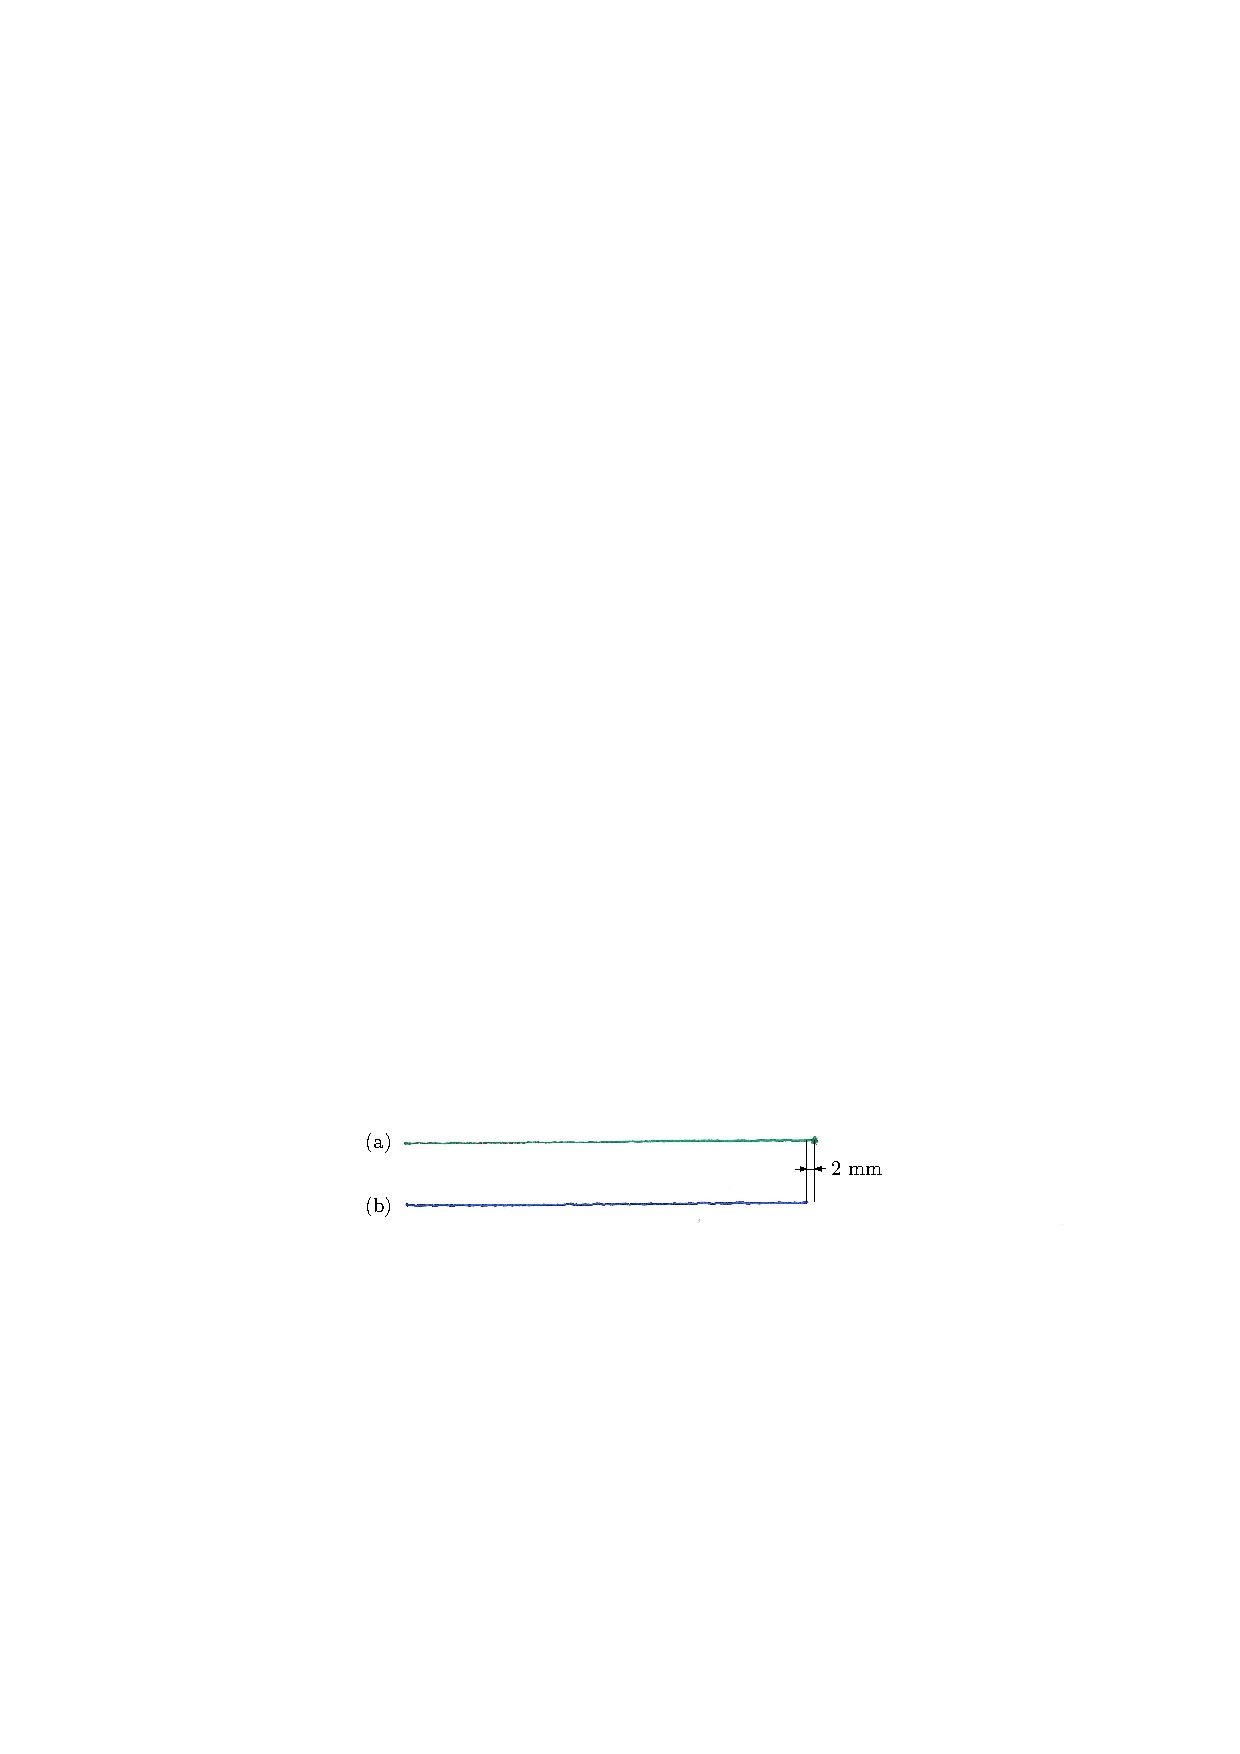
\includegraphics{resultatLinia}
		\caption{Dibuix d'una línia recta de 100 mm.}
		\label{fig:linia}
	\end{figure}
	Com es pot observar a la imatge s'ha realitzat la prova dues vegades. En primer, lloc s'ha relitzat la línia verda (a) i s'ha comprovat que la mida és de 102 mm enlloc dels 100 esperats. Això és degut a la mala calibració de l'aparell, i s'ha tornat a calibrar amb l'ajuda d'un peu de rei. Amb el nou diàmetre s'ha pogut realitzar una segona línia, la blava (b), que, aquest cop sí, mesura 100 mm. 
	
	\item La següent prova consisteix en la realització d'un quadrat de 100 mm de costat. Aquest cop s'ha realitzat amb el robot ja calibrat, tant el diàmetre de les rodes com la distància entre aquestes i el centre. El resultat és el següent:
	\begin{figure}[H]
		\centering
		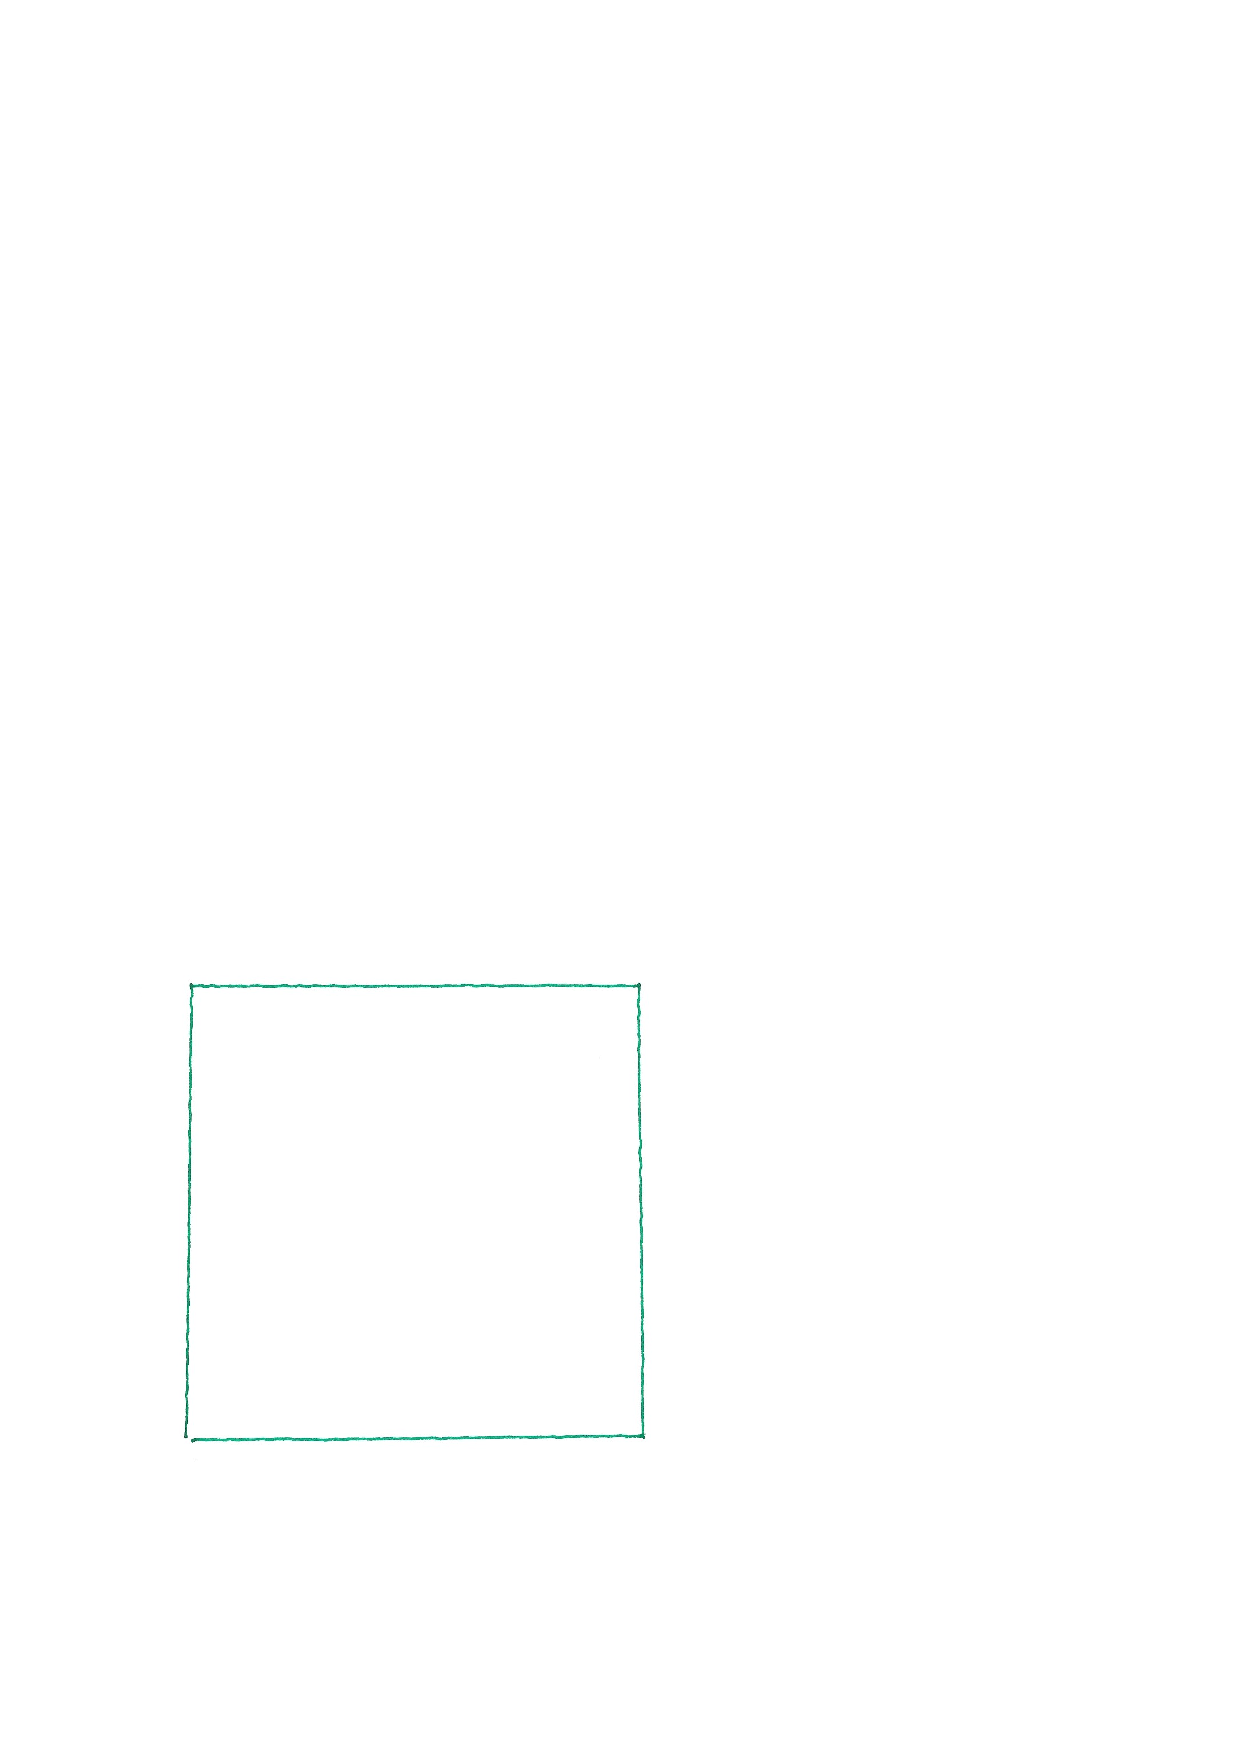
\includegraphics{resultatQuadrat}
		\caption{Dibuix d'un quadrat de 100 mm de costat.}
		\label{fig:quadrat}
	\end{figure}
	Es pot observar que el resultat és bo, tot i que no acaba de tancar la silueta del tot com s'observa a la cantonada inferior esquerra. Es dedueix que aquest error que es comet als vèrtexs, ja que tots els costat mesuren 100 mm. Això és degut a l'acumulació de l'error que es comet. No és un sistema perfecte, i els passos no són infinitessimals, per la qual cosa sempre es comet un petit error. Aquest error és molt més visible als angles que no pas a les rectes, ja que a les línies rectes només afecta a les distàncies, mentre que l'altre distorssiona tota la imatge. 
	
	\item A partir d'aquí ja s'ha treballat amb figures més complicades creades amb Inkscape. Primer s'ha realitzat una estrella i s'ha obtingut el següent resultat:
	\begin{figure}[H]
		\centering
		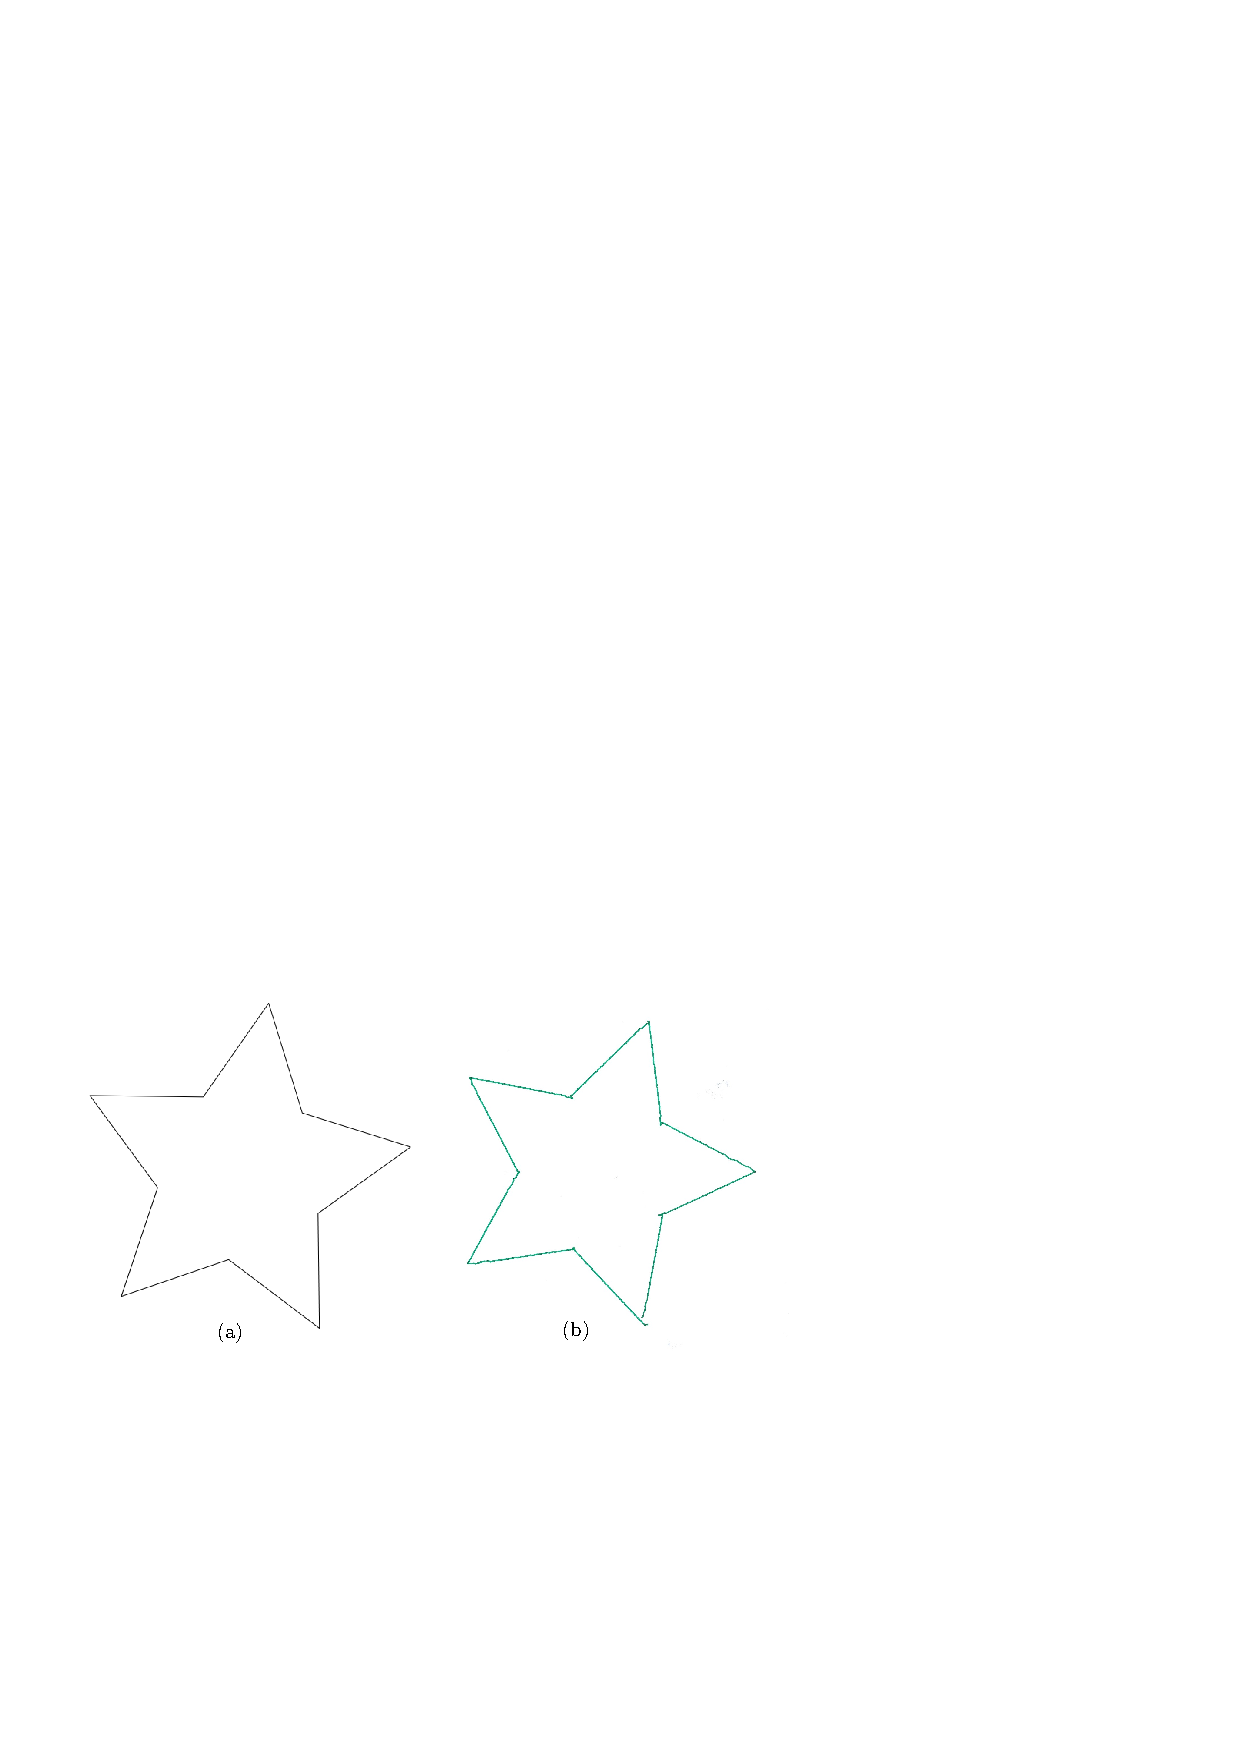
\includegraphics[scale=0.9]{resultatEstrella}
		\caption{Dibuix d'una estrella (Dibuix en Inkscape (a), Dibuix del robot (b)).}
		\label{fig:estrella}
	\end{figure}
	Com es pot veure, la respresentació és bastant acurada, tot i que es torna a observar l'error en l'angle de gir. En aquest cas, però, al girar en sentit invers a cada vèrtex es compensa en certa mesura aquest error i la distorsió de la imatge és baixa. Es pot veure que tampoc s'aconsegueix tancar el contorn de la figura. 
	
	\item Per comprovar el funcionament de les comandes G02 i G03 s'ha realitzat una figura simple amb l'ajuda de l'aplicació creada. Aquesta figura es basa en una línia recta, mitja circumferència realitzada amb un moviment G02 en sentit horari, mitja circumferència realitzada amb una comanda G03 en sentit antihorari i dues rectes més que tanquen el contorn. El resultat és el segûent:
	\begin{figure}[H]
		\centering
		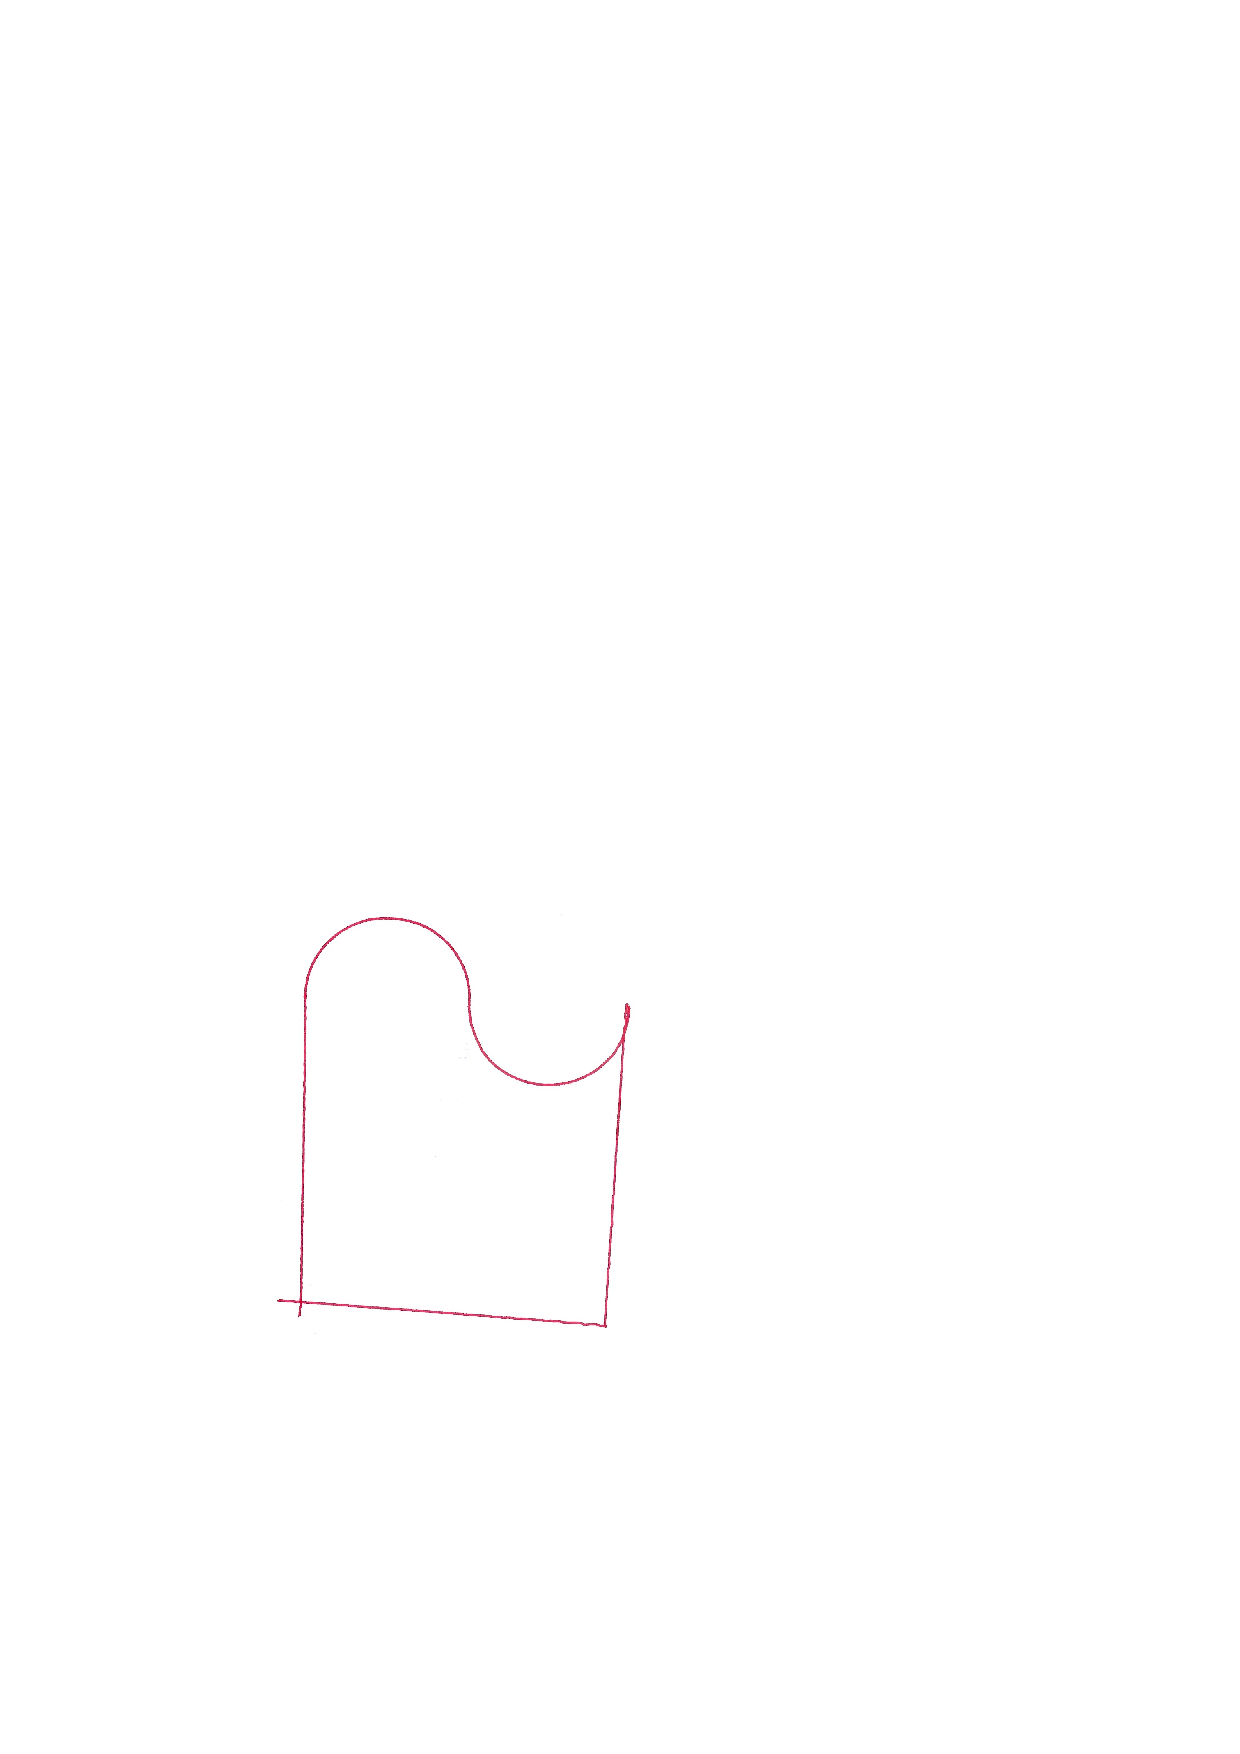
\includegraphics{resultatFuncionara}
		\caption{Dibuix d'una figura amb arcs de circumferència.}
		\label{fig:funcionara}
	\end{figure}	
	L'error en l'angle es manté aproximadament igual que a les figures anteriors. Aquí, però, es pot observar un moviment horitzontal no desitjat de la punta del retolador que es presenta al final del segon arc de circumferència. Això pot ser causat pel joc del retolador, i pel mal centratge de la rotació.
	
	\item Per acabar, s'ha representat una lletra \textit{i} per tal de provar figures més complicades i moviments de posicionament. Després de crear-la a l'Inkscape s'ha aconseguit aquest resultat:
	\begin{figure}[H]
		\centering
		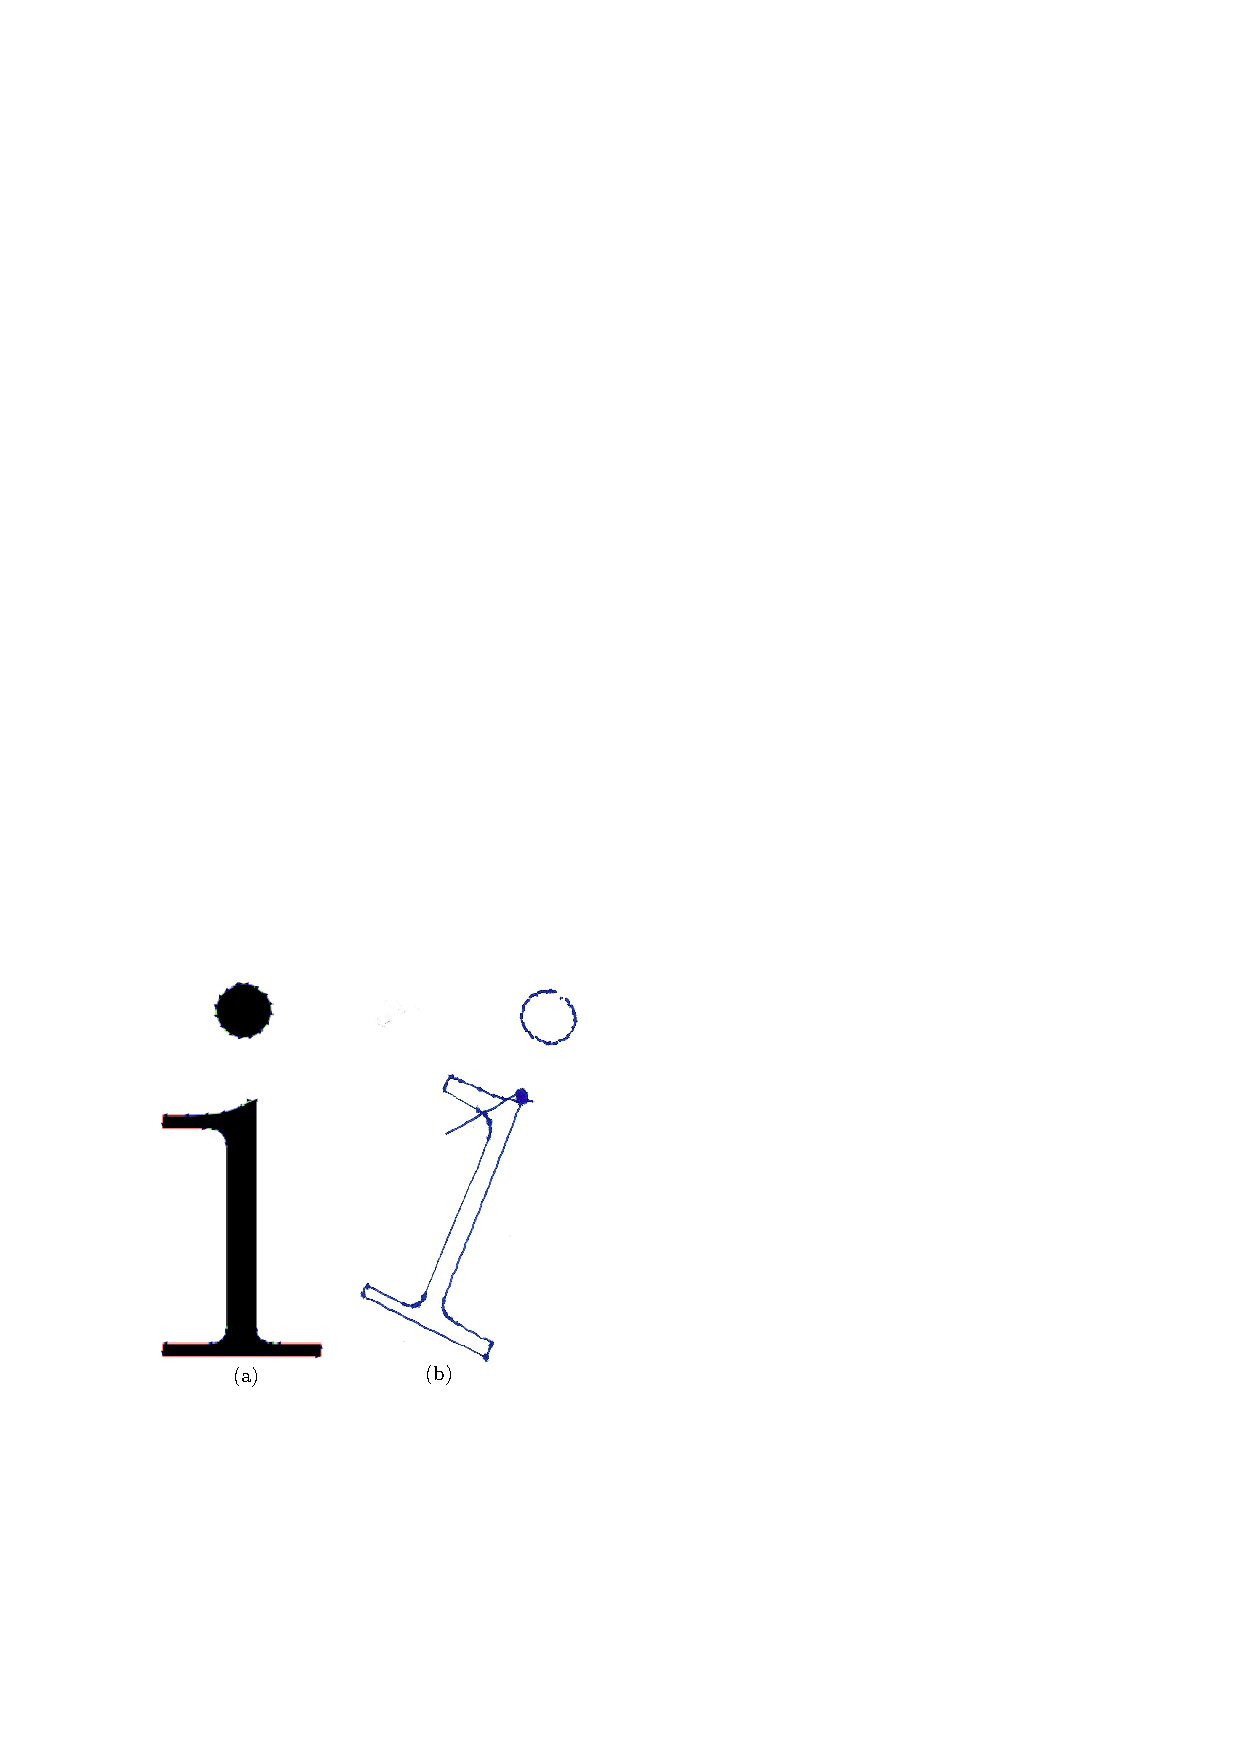
\includegraphics{resultatLletra}
		\caption{Dibuix d'una lletra \textit{i} en Inkscape (a) i dibuixada pel robot (b).}
		\label{fig:Lletra}
	\end{figure}
	La forma de la lletra es manté bastant similar a l'original, es pot veure com s'ha pogut tancar el cos i que manté una forma molt aproximada. Cal destacar, però, que hi ha diferents errors. En primer lloc, cal dir que la línia diagonal que no pertany al dibuix s'ha creat degut a un error de muntatge, ja que a l'acabar s'ha desenganxat l'accionador del servo que s'encarrega d'aixecar el retolador. Aquest error s'ha solucionat enganxant aquest accionador amb cola de contacte. Aquí el principal error s'acumula a la realització del punt de la \textit{i}. Al crear la trajectòria en Inkscape, aquest no detecta el punt com una circumferència perfecta i la crea a partir de molts arcs de petites dimensions. Això provoca constants aturades del robot per tal de realitzar rotacions molt petites i l'error que s'acumula és molt gran. Al ser la primera part que es dibuixa, distorsiona tota la imatge que queda desviada. Això s'observa al punt, veient que no s'acaba de tancar la silueta per la part superior. A l'arribar a l'últim punt de la circumferència que dibuixa el robot, aquest gira 90 graus, però com que aquest punt no coincideix amb l'inicial, la direcció del robot no és l'esperada. Això provoca aquesta desviació. 
	
	Per comprovar-ho, s'ha modificat el GCode i s'ha definit el punt com una cirumferència perfecta creada a partir de dos arcs de mitja cirumferència. El resultat és el següent:
	\begin{figure}[H]
		\centering
		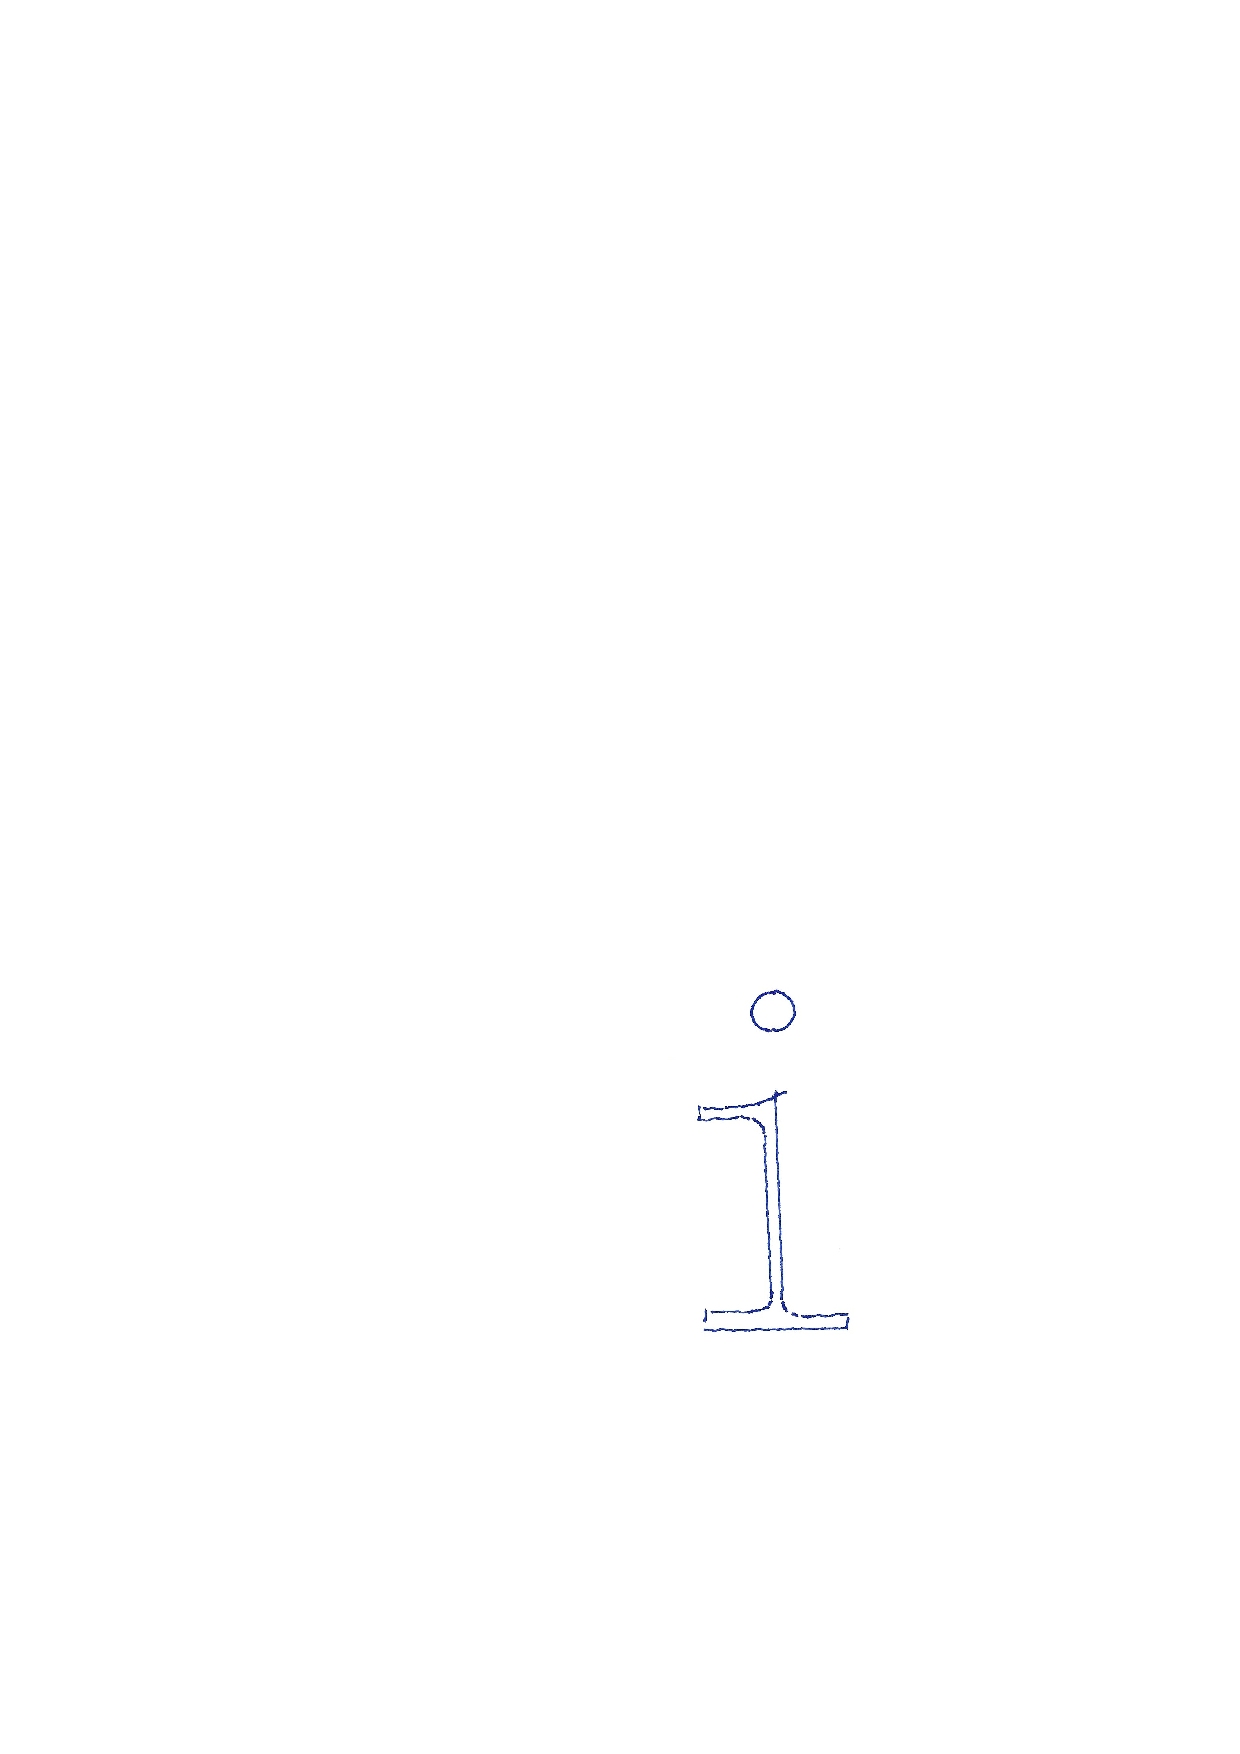
\includegraphics{resultatLletra2}
		\caption{Dibuix de la lletra \textit{i} millorat.}
		\label{fig:Lletra2}
	\end{figure}
	El canvi és clar: l'error més elevat es comet al realitzar els petits moviments circulars del punt. Així s'aconsegueix un punt més definit i una lletra més ben posicionada.
	
	Els errors que es poden observar es localitzen principalment en el calibratge del robot. A part dels aspectes que s'han esmentat, també existeixen possibles errors de disseny i construcció que poden provocar aquests errors, per exemple un mal centratge de les rodes, que aquestes no siguin perfectament perpendiculars a l'eix, que existeixi un petit lliscament entre l'eix i la roda o la deformació de les juntes, que actuen com a neumàtic, que pot ser diferent al llarg del recorregut. També és possible que a causa de la fricció algún pas del motor no es realitzi com toca i això provoqui aquest error.  
	
	Per millorar els errors de disseny o vibracions del motor caldria redissenyar les peces, adquirir nous components amb millors prestacions i millorar els materials que el composen, per exemple. Això reduiria l'error en llaç obert considerablement. Per altra banda, es podrien estudiar les diferents vies que existeixen per tancar el llaç de control i intentar corregir aquest error com s'explica més endevant en l'apartat \ref{sec:treballsfuturs} de possibles treballs futurs, ja que no entra a l'abast d'aquest projecte. 
	
	
	
\end{itemize}



